% Compact PGFPlots panel for sampled qldpc_38_4_5_cap7 BSC correction-class derivative.
% Requires \usepackage{pgfplots} and \pgfplotsset{compat=1.18}.
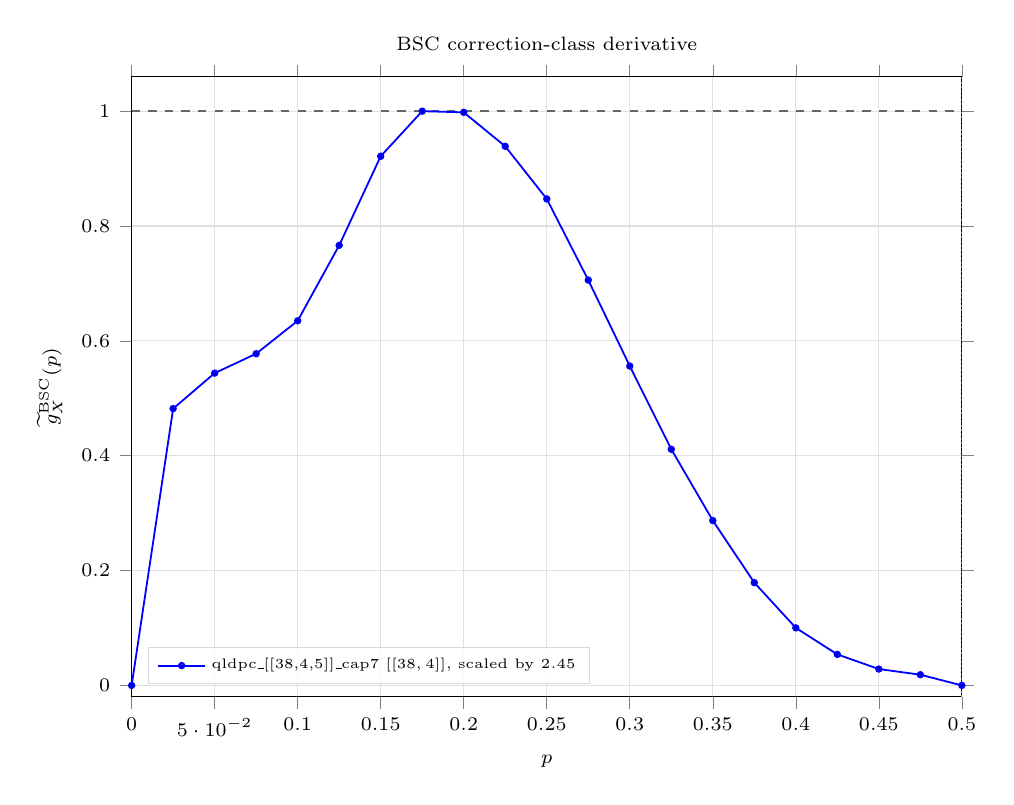
\begin{tikzpicture}
\begin{axis}[
  name=scaledBSCGEXITQldpc3845Cap7Axis,
  width=\linewidth,
  height=0.78\linewidth,
  title={BSC correction-class derivative},
  title style={font=\scriptsize},
  xlabel={$p$},
  ylabel={$\widetilde g_X^{\rm BSC}(p)$},
  xmin=0, xmax=0.5,
  ymin=-0.02, ymax=1.06,
  grid=both,
  major grid style={black!12},
  minor grid style={black!6},
  tick align=outside,
  tick label style={font=\scriptsize},
  label style={font=\scriptsize},
  legend cell align={left},
  legend style={draw=black!15, fill=white, fill opacity=0.82, text opacity=1, at={(0.02,0.02)}, anchor=south west, font=\tiny},
]
\addplot[black!60, densely dotted, line width=0.55pt, forget plot] coordinates {(0.5,-0.02) (0.5,1.06)};
\addplot[black!60, dashed, line width=0.55pt, forget plot] coordinates {(0,1) (0.5,1)};
\addplot+[color=blue, mark=*, mark size=1.0pt, line width=0.65pt]
coordinates {(0,0) (0.025,0.482058539208) (0.05,0.54382798378) (0.075,0.577644169978) (0.1,0.635023402432) (0.125,0.766383121249) (0.15,0.921538720343) (0.175,1) (0.2,0.997989737272) (0.225,0.938784830047) (0.25,0.847219709115) (0.275,0.705919868497) (0.3,0.556183529733) (0.325,0.411294009519) (0.35,0.287097750754) (0.375,0.17899215876) (0.4,0.100239804046) (0.425,0.05402524402) (0.45,0.0285123199666) (0.475,0.0186480121883) (0.5,0)};
\addlegendentry{qldpc\_[[38,4,5]]\_cap7 $[[38,4]]$, scaled by $2.45$}
\end{axis}
\end{tikzpicture}
